Following Run 2, a staged installation of Gas Electron Multipliers (GEMs) \cite{GEM} began as part of the Phase 2 upgrades to the muon system. Located in the very forward regions of each ME and complementing the CSCs, the GEMs cover the pseudorapidity range of $1.5<|\eta|<2.8$ and are labeled GE$\pm$1/1 (installed during LS2), GE$\pm$2/1 (installation slated for year-end technical stops in Run 3), and ME$\pm$0 (installation slated for LS3). Each GEM detector consists of a triple-layer of copper-cladded polyimide foil into which are etched \SI{70}{\micro \meter} holes spaced \SI{70}{\micro\meter} apart, in a hexagonal geometry, as can be seen in the diagrams in Figs.~\ref{fig:GEMDiagram} and~\ref{fig:GEMDiagram2} (left). A 70 \% Ar and 30 \% CO$_2$ gas mixture fills mm-sized gaps between the foil layers and a voltage is applied is steps ranging from \SI{-3200}{V} to ground (see Fig.~\ref{fig:GEMDiagram2}, right). The foil layers are sandwitched between a drift PCB and a readout PCB with 3072 radial strips. A total of 144 GEM chambers were installed during LS2 occupying the GE$\pm$1/1 station/ring, with the remaining chambers, ME$\pm$0 and GE$\pm$2/1 to be installed in LS3. 

\begin{figure}[H]
    \centering
    {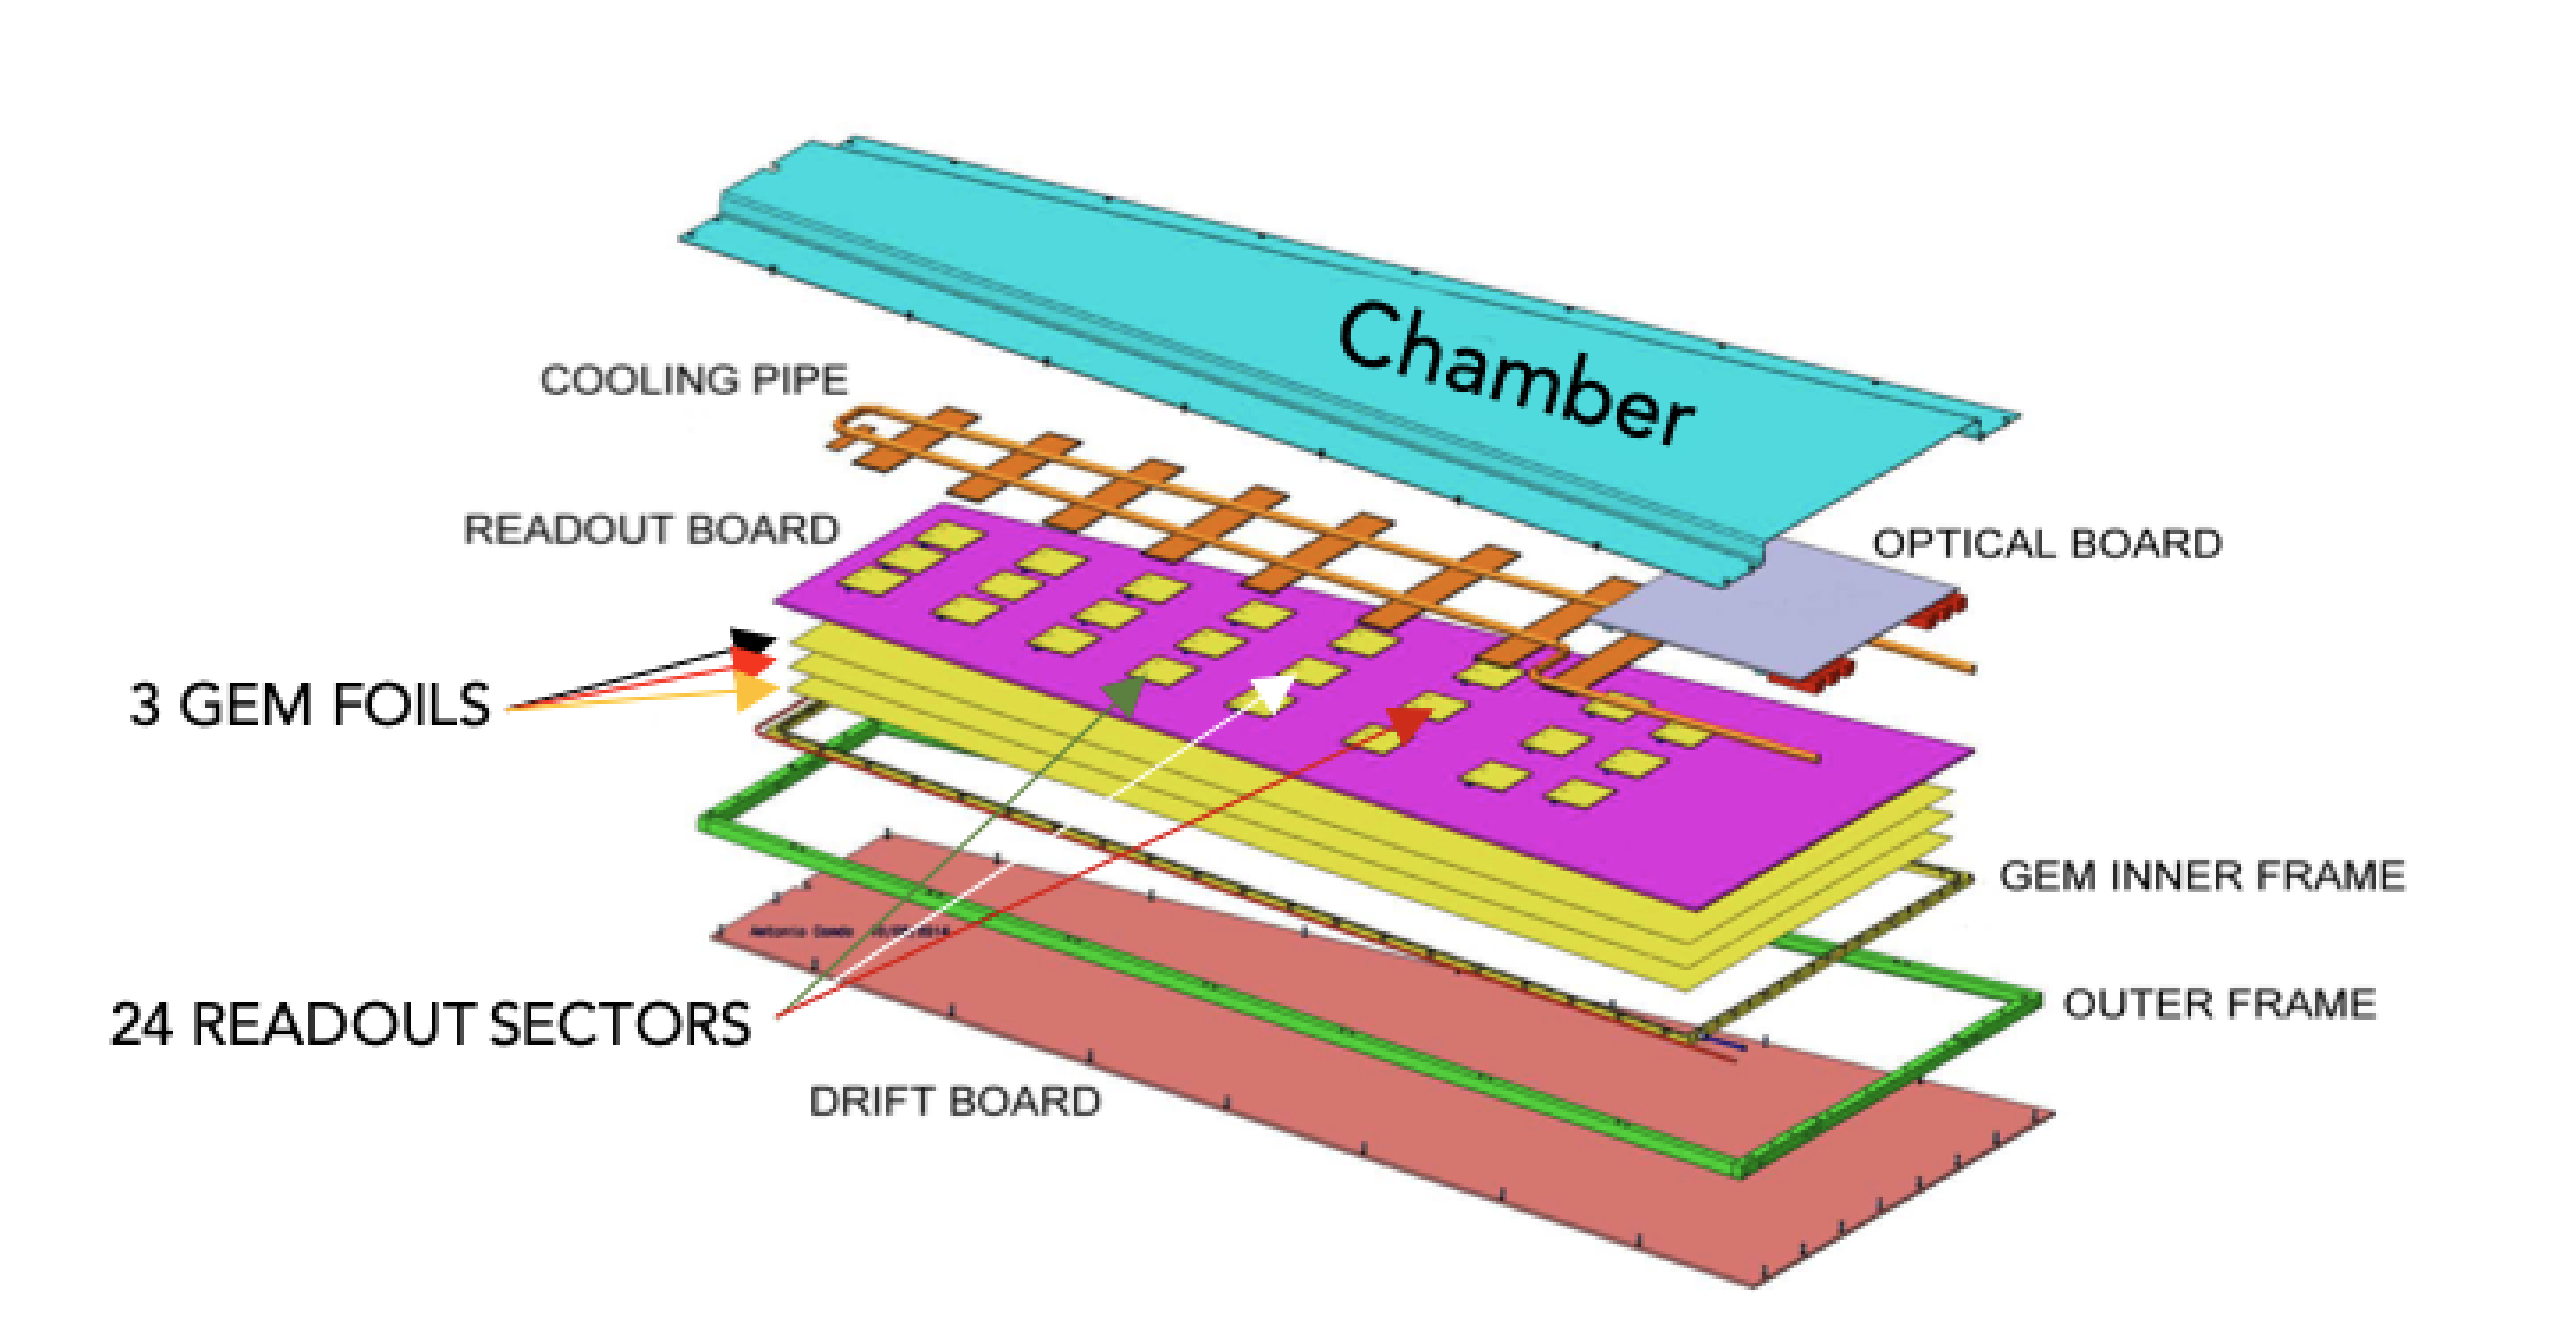
\includegraphics[width=\textwidth]{Images/CMS/GEMDiagram.png}}
    \caption{An exploded view of a GEM chamber.}
    \label{fig:GEMDiagram}
\end{figure}

\begin{figure}[H]
    \centering
    {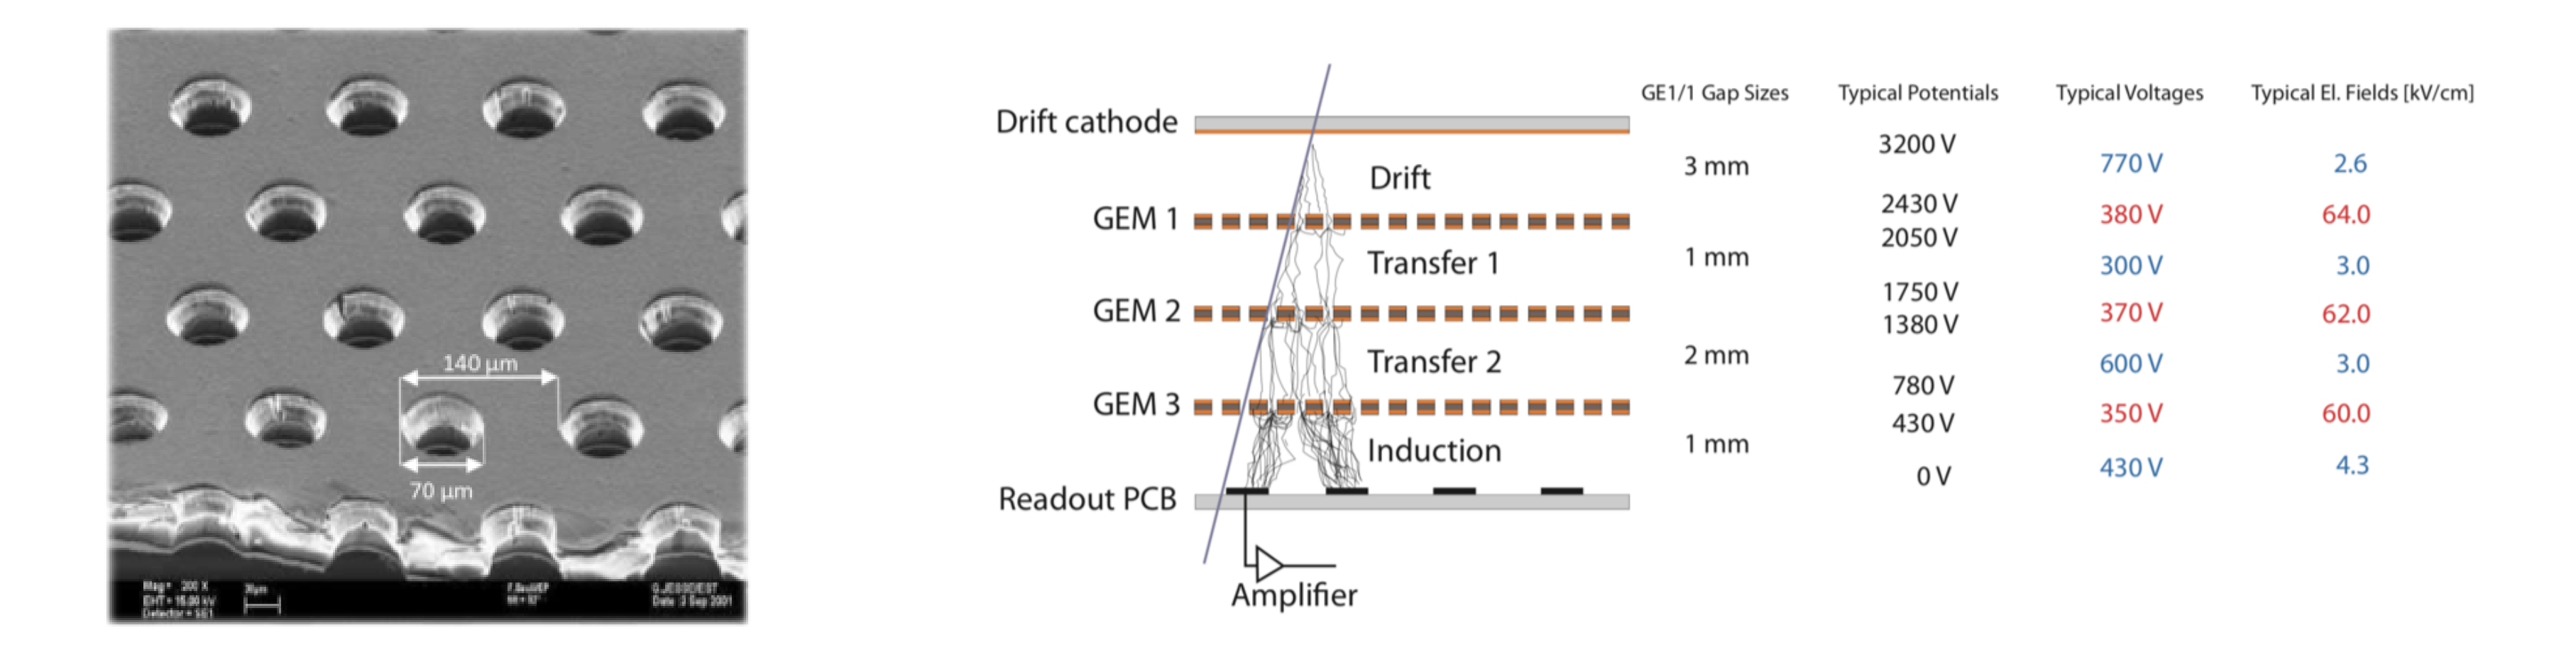
\includegraphics[width=\textwidth]{Images/CMS/GEMDiagram2.png}}
    \caption{Left: a photograph of the micron-scale holes in the GEM foil. Right: The typical voltages in each layer of a GEM chamber.}
    \label{fig:GEMDiagram2}
\end{figure}